% begin module horizontal-line-test
\begin{frame}
Question: How can we tell from the graph of a function whether it is one-to-one or not?

Answer: Use the horizontal line test.

\begin{proof}[The Horizontal Line Test]
A function is one-to-one if and only if no horizontal line intersects it more than once.
\end{proof}

\begin{tabular}{cc}
\psset{xunit=0.7cm, yunit=0.7cm}
\begin{pspicture}(-5, -5)(5,5) 
\psframe*[linecolor=white](-5,-5)(5,5) 
\psaxes[ticks=none, labels=none]{<->}(0,0)(-3,-3)(3,3)
%Function formula: 1/2 (x)+1/2 
\psplot[linecolor=red, plotpoints=1000]{1}{2}{0.5 x 0.5 mul add } %Function formula: (x)^{3} 
\psplot[linecolor=red, plotpoints=1000]{-1}{1}{x 3 exp } %Function formula: 3/2 (x)+1/2 
\psplot[linecolor=red, plotpoints=1000]{-2}{-1}{0.5 x 1.5 mul add }
\end{pspicture} 
%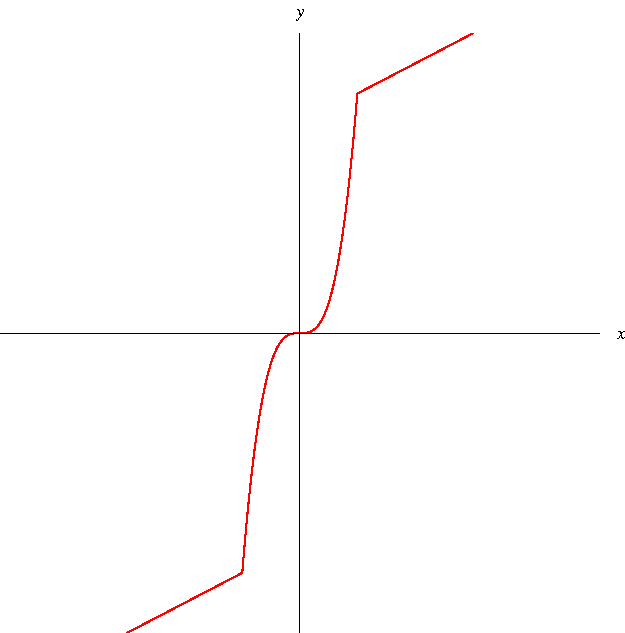
\includegraphics[height=4cm]{inverse-functions/pictures/07-01-onetoone.pdf} 
 %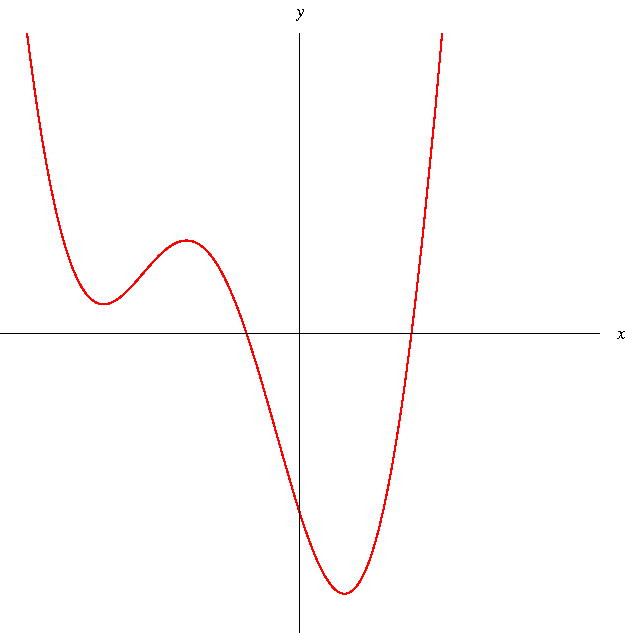
\includegraphics[height=4cm]{inverse-functions/pictures/07-01-notonetoonea.pdf}%
&%
\uncover<handout:0| 2->{%
\psset{xunit=0.7cm, yunit=0.7cm}
\begin{pspicture}(-5, -5)(5,5) 
\psframe*[linecolor=white](-5,-5)(5,5) 
\psaxes[ticks=none, labels=none]{<->}(0,0)(-3,-3)(3,3)
 %Function formula: -2/5+((6/5+x)^{2}) ((x) (x))-6/25 ((6/5+x)^{2})- (((6/5+x)^{2}) (x)) 
 \psplot[linecolor=red, plotpoints=1000]{-2}{1.5}{x x 1.2 add 2 exp mul -1 mul x 1.2 add 2 exp -0.24 mul add x x mul x 1.2 add 2 exp mul add -0.4 add }
 \uncover<3->{
 \psline[linestyle=dashed](-3, 1)(3, 1)
 }
 \end{pspicture} 
}
\\
\uncover<2->{\alert<handout:0| 2>{One-to-one}} &
\uncover<3->{\alert<handout:0| 3>{Not one-to-one}}
\end{tabular}
\end{frame}
% end module horizontal-line-test
